\documentclass[tikz,border=3pt]{standalone}
\usepackage{tikz}
\usepackage{amsmath}
\usepackage{pgfplots}
\pgfplotsset{compat=1.18}

\begin{document}
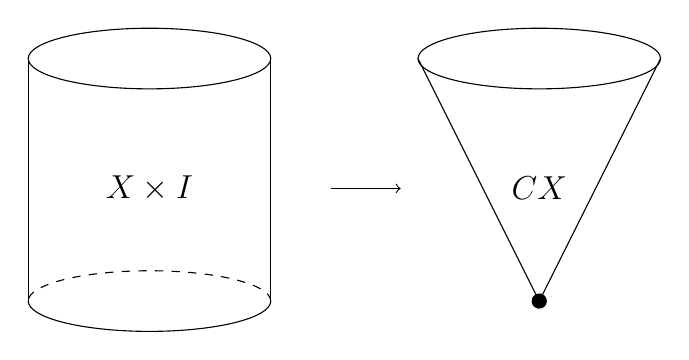
\begin{tikzpicture}[
    scale=1.1,
    every node/.style={font=\large}
]

% Cylinder X x I
\draw (0,2) ellipse (1.4 and 0.35);
\draw (-1.4,2) -- (-1.4,-0.8);
\draw (1.4,2) -- (1.4,-0.8);

\draw (-1.4,-0.8)
    arc[start angle=180,end angle=360,
        x radius=1.4,y radius=0.35];

\draw[dashed]
    (1.4,-0.8)
    arc[start angle=0,end angle=180,
        x radius=1.4,y radius=0.35];

\node at (0,0.5) {$X\times I$};

% Arrow
\draw[->] (2.1,0.5) -- (2.9,0.5);

% Cone CX
\draw (4.5,2) ellipse (1.4 and 0.35);
\draw (3.1,2) -- (4.5,-0.8);
\draw (5.9,2) -- (4.5,-0.8);
\fill (4.5,-0.8) circle (2.5pt);

\node at (4.5,0.5) {$CX$};

% % Definition
% \node[anchor=west] at (6.0,0.5)
%     {$CX := X\times I / X\times\{0\}$};

\end{tikzpicture}
\end{document}